\chapter{Visual Mappings And Interactive Functionality}
This chapter describes different visualizations and interaction methods developed based on the visualization requirements and data abstraction discussed in Chapter 2 and 4. In general, the visualization is divided into two parts: Session visualization which visualize movement in one particular session and Summary visualization which visualize movement over different sessions. Both visualization is organized in an application where user can select player and sessions he has played. At first, the earlier version of visualization will be explained. This earlier version is not used in the final version since it's difficult to get any information intuitively. Then, each type of visualization and its interaction used in the final version will be discuss. In the end, the application which encapsulate both visualization will be presented.

\section{Early version of the Visualization}
The first visualization method chosen to represent \ref{t11} and \ref{t12} is line chart. In this approach, the x area is shown as a horizontal axis and the number of events shown in vertical axis with the line signify the changes of number of events for different x area unit. In the log file, each event is recorded with distinct 3D coordinate location. The x value from this coordinate is a decimal, therefore visualizing each one of this x value will require a lot of space. To solve this, the events are then grouped by the rounded x value. In figure 5.1 below, Negative events are shown in red line and Positive events are shown in blue line. As we can see, it's possible to know which event type happened more in a certain x unit, however it is difficult to see how big a percentage is it compare to total number of events happened in the same x unit.

\begin{figure}
\centering
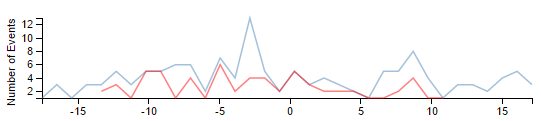
\includegraphics[width=100mm]{linechart.png}
\caption{First visualization version for \ref{t13} and \ref{t14} using Scatter Plot}
\end{figure}

\begin{figure}
\centering
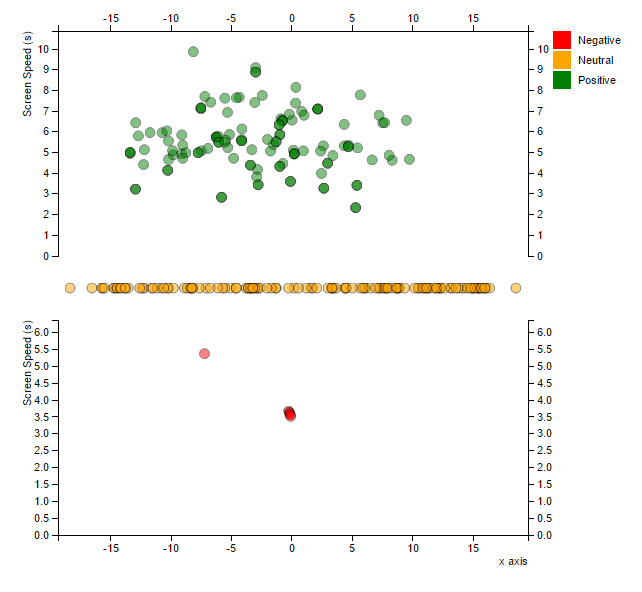
\includegraphics[width=100mm]{scatterplot.png}
\caption{First visualization version for \ref{t11} and \ref{t12} using Line Chart}
\end{figure}

Visualization method chosen to represent \ref{t13} and \ref{t14} is scatter plot. At first, each event type is presented in three different chart area: top are for Positive events, middle are for Neutral events, and bottom area for Negative events. Similar to the line chart, the x value from the 3D coordinate location are represented in horizontal x axis. However, the vertical axis here represent the screen speed. For the scatter plot, each event is shown as a plot in the chart area according to it's x value and screen speed as shown in figure 5.2. Even though similar pattern can be seen on the scatter plot, occlusion problem prevent users to know how many event are actually happened in a certain x area.

\section{Session Visualization}
The Session Visualization visualizes events within a game session. Basically, the requirement can be split into two: (i) knowing the distribution of events and movements (ii) knowing the distribution of events, movements and screen speed. Therefore, there are two chart developed to meet these requirements: stacked area for (i) and heatmap for (ii), each of which will be explain in details in this section.

\subsection{Stacked Graph}
Build on layered area graph, Stacked Graph is widely used to visualize evolution of variable over times such as document theme \cite{havre}, box office movie revenue\footnote{\url{http://www.nytimes.com/interactive/2008/02/23/movies/20080223_REVENUE_GRAPHIC.html?_r=0}}, listening history in Last.fm \cite{byron},etc., Stacked Graph is chosen because its ability to show individual value of a variable, the difference between values of different variables as well as the total of overall value. In my approach, instead of using this metaphor to show evolution over time, it is used to show distribution of events over spatial coordinate \ref{t11}\ref{t12} as shown in figure 5.3. Here, the horizontal axis represents x coordinate and vertical axis represents number of events. Each event type is represented as an area with different color: Red (Negative), Yellow (Neutral), and Green (Positive). To help user understand better the distribution of each event type, different layout of stacked graph is provided: 
\begin{enumerate}
  \item Linear: zero y axis is used as the baseline, with the stack ordered from bottom as negative, neutral, positive.
  \item Silhouette: the graph is centered as in streamgraphs.
  \item Positive: zero y axis is located at the top of the chart and is used as the baseline with the stack ordered from top as positive, neutral, negative.
  \item Neutral-Negaive: zero y axis is located in the middle of the chart. Neutral and Positive event is shown on the positive area of y axis and Negative is shown on the negative area of y axis.
  \item Positive-Neutral: zero y axis is located in the middle of the chart. Positive event is shown on the positive area of y axis, while Neutral and Negative is shown on the negative area of y axis.
\end{enumerate}

\begin{figure}
\centering
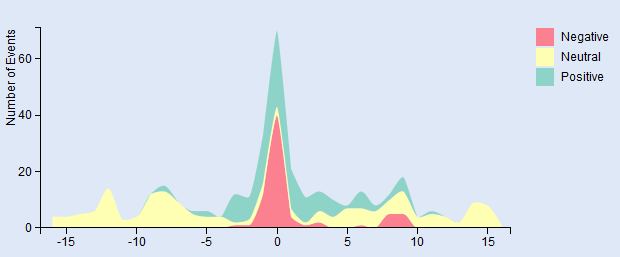
\includegraphics[width=100mm]{stackedgraph_linear.png}
\caption{Stacked Graph with Linear Layout}
\end{figure}

\begin{figure}[htp] % not h only
\centering
\subfloat[Silhouette]{%
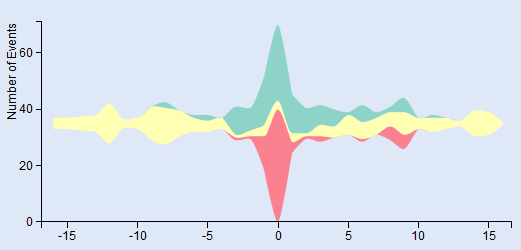
\includegraphics[width=0.4\textwidth]{stackedgraph_silhouette.png}%
\label{fig:silhouette}%
}\hfil
\subfloat[Positive]{%
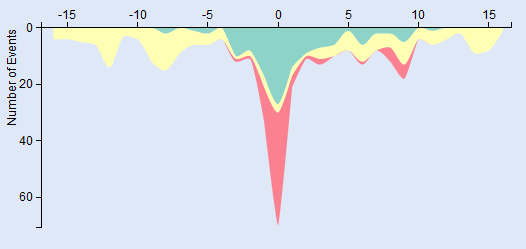
\includegraphics[width=0.4\textwidth]{stackedgraph_positive.png}%
\label{fig:positive}%
}

\subfloat[Neutral-Negative]{%
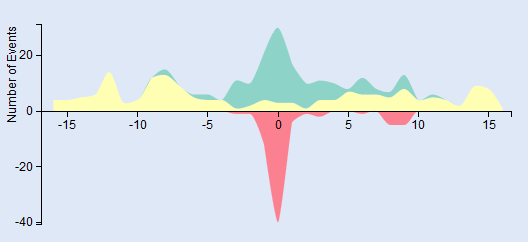
\includegraphics[width=0.4\textwidth]{stackedgraph_neutral_neg.png}%
\label{fig:neutral-negative}%
}\hfil
\subfloat[Positive-Neutral]{%
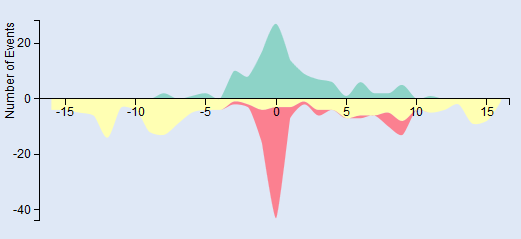
\includegraphics[width=0.4\textwidth]{stackedgraph_positive_neutral.png}%
\label{fig:positive-neutral}%
}

\caption{Different Layout of the Stacked Graph representing number of events over x-axis}
\end{figure}

For each stacked graph layout, user can choose which object type to show on the graph \ref{t15}. Options are available as radio button on top of the chart. Therefore, choosing Bonus will show only Positive and Neutral events, choosing Obstacle will show only Neutral and Negative events, and choosing Enemy will show all event type.

\subsection{Heat Map}
\begin{figure}
\centering
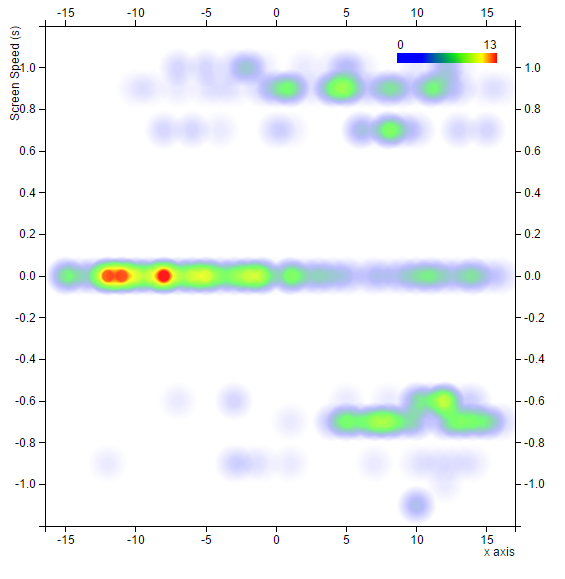
\includegraphics[width=100mm]{heatmap.png}
\caption{Heatmap}
\end{figure}
Heat Map is a quite popular visualization method nowadays due to its ability which allows user to see variable with the highest value at one glance. Most of the time, heatmap is implemented on geographical map to represent variable value over certain area on map, i.e: Natural Disaster Risk by Location\footnote{\url{http://www.rms.com/}}, population density\footnote{\url{https://en.wikipedia.org/wiki/Population_density}}, Number of picture taken in an area\footnote{\url{http://sightsmap.com/}}, etc. Heat map is also used to track eye movement or mouse click on a website, and representing DNA microarray data in the form of cluster heat map\cite{friendly}. Heat map uses color gradation to represent the hotness level of a variable. Usually, red color is used to represent the high value (hot) and blue is used to represent the low value (cold). However, other color combination can also be used. To represent distribution of events and screen speed over x axis \ref{t13}\ref{t14}, the events are first grouped based on it's x value and normalized screen speed. The number of events is then represented as heat map on the graph with highest number of events in red color. Normalized screen speed is represented as vertical axis and x value is represented as horizontal axis. Using the same approach used in scatter plot chart, each event type is presented in different area: top for positive, middle for neutral, and bottom for negative. For Neutral events, the screen speed is not calculated since it basically mean an object has been avoided or missed. For Negative events, the screen speed is represented in negative to show that it's an uncalculated movement. For the heatmap, user can also choose to show a specific object \ref{t16} by clicking the radio button associated with the desired object.

\section{Summary Visualization}
The Summary Visualization fulfills the requirements concerning movement evolution over time (\textit{T}2). In this case, a single session is considered as a single time point. Since user are interested in evolution over a certain x-area, the visualization are divided into sections of x-area. There are two ways of division: by the range of x-area and by the number of events within an area. The following explains the two approach and its interaction technique in details.

\subsection{Visualization by range of x-area}
To fulfill \ref{t21} and \ref{t22}, a streamgraph metaphor is chosen to show evolution of movement (represented by events) over time. Similar to the approach chosen in the Session visualization, the horizontal axis represent x coordinates of events. The vertical axis represent different sessions with the earliest one shown at the bottom and the latest one shown on the top. The x axis is then divided into sections of the same range based on user input. For each section, events are then filtered to the one which happened within the section x boundary. The filtered events are grouped based on session number and event type. Number of events within this group is then presented in vertical streamgraph layout with event type represented using the same color used in the Session visualization (Figure  \ref{fig:type1_not_clustered}). 

Shown in figure \ref{fig:type1_section} a section in the chart. Here, the lower x boundary is -20 and the upper x boundary is -7.33. Within this area, the evolution of events throughout all session can be seen\ref{t22}. It is also possible to see which session has the most or least number of events by comparing the total length of all event type in one session. 

\begin{figure}
\centering
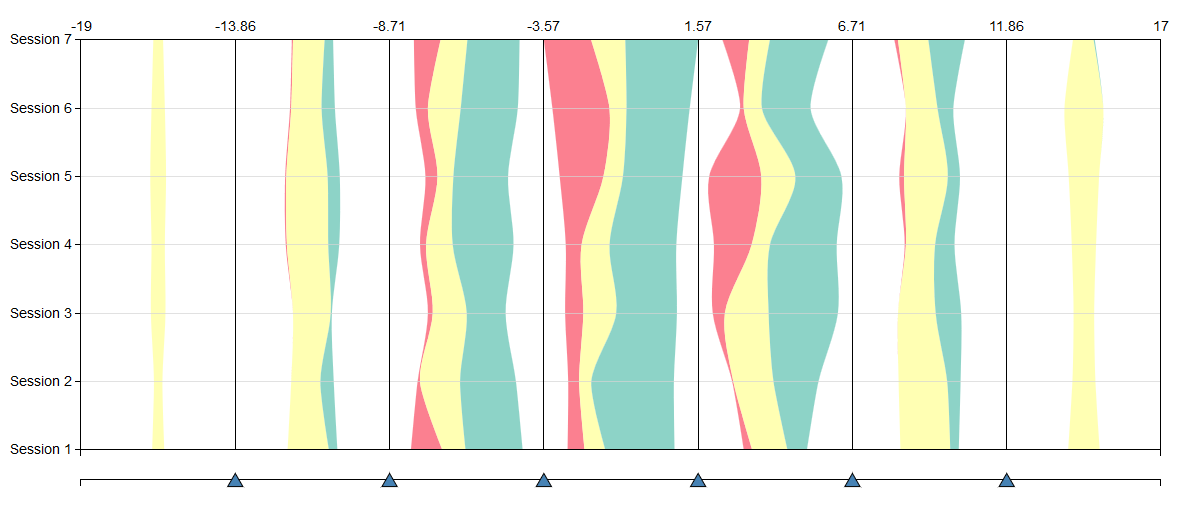
\includegraphics[width=130mm]{summary_not_clustered.png}
\caption{Summary Chart divided by range of x-area}
\label{fig:type1_not_clustered}
\end{figure}

\begin{figure}
\centering
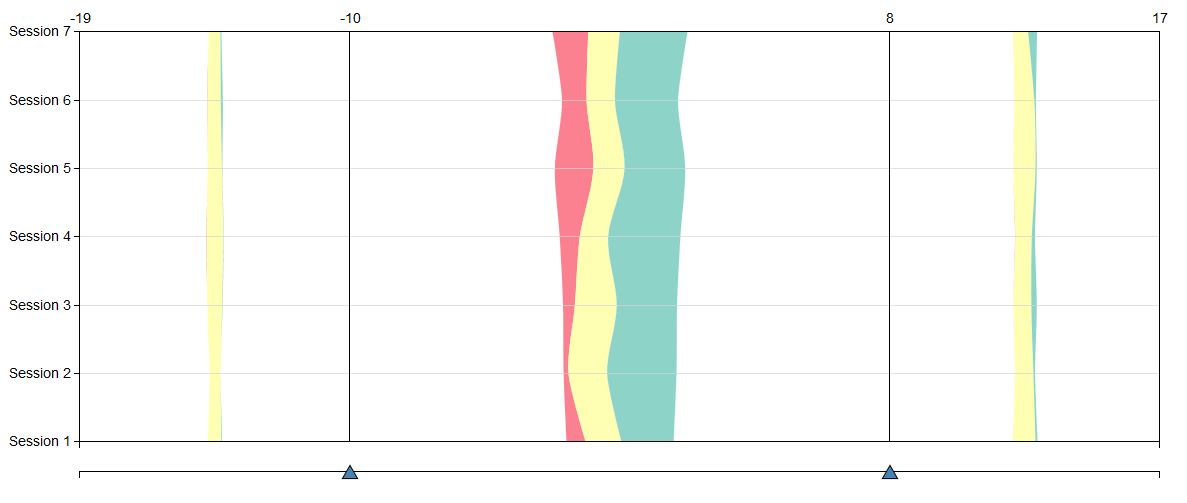
\includegraphics[width=130mm]{summary_clustered.png}
\caption{Summary Chart divided by range of x-area, clustered with threshold = 4}
\label{fig:type1_clustered}
\end{figure}

\begin{figure}
\centering
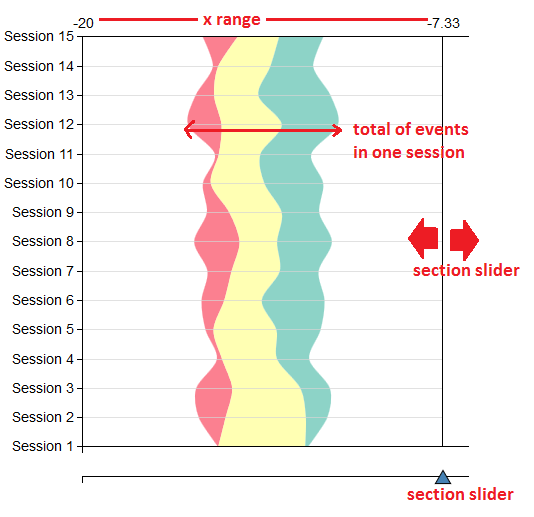
\includegraphics[width=80mm]{section.png}
\caption{A section in Summary Visualization}
\label{fig:type1_section}
\end{figure}

By default, once a user input the desired x-range, the clustering algorithm as explained in Chapter 4 is applied\ref{t27}. Thus it is possible that the number of sections shown in the visualization are fewer than initially inputted. Shown in figure \ref{fig:type1_clustered} a clustered version of figure \ref{fig:type1_not_clustered}. Here the first and last two sections are merged into one section. Such the case with the three sections in the middle.

\subsection{Visualization by number of events}
This second type of Summary Visualization uses the same approach explained previously. However, a section is calculated based on the total number of positive and negative events instead of the range of x-axis \ref{t24}\ref{t25}. Therefore, based on the distribution of positive and negative events, one section in the chart may have bigger x-range than the other section. Only by comparing the size of sections, it's possible to know in which area most of the events are concentrated. Figure \ref{fig:type2} shows that the events are more concentrated in the middle area of the screen. Here, it can be concluded that on the far right and far left of the screen, there are more neutral events compare to the middle area.

\begin{figure}
\centering
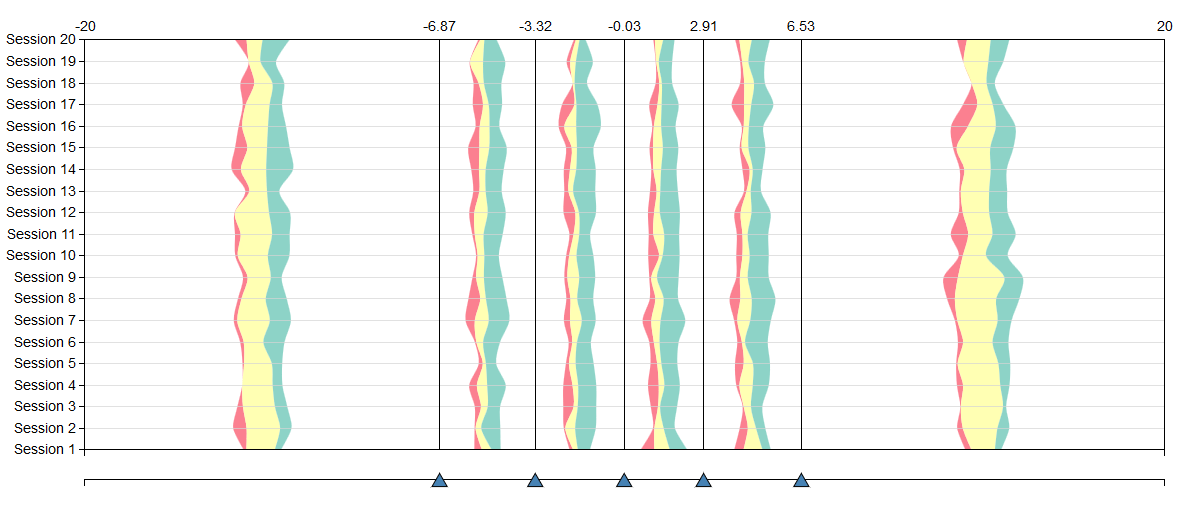
\includegraphics[width=130mm]{summary_type2.png}
\caption{Summary Chart divided by number of events}
\label{fig:type2}
\end{figure}

\subsection{Interaction Technique}
On top of the chart, an interaction bar is provided where user can interact with and change some variable in the chart. In the first panel of the interaction bar (figure \ref{fig:interaction_bar}), a slider which serves two function is provided. First, as an x-range input, second as a number of events input. This two functions can be activated by turning the switch on/off. When the switch is ON, the slider will act as an x-range input. The value on the slider basically define the number of sections on the chart. The more number of sections, the smaller the x-range. When the switch is OFF, the slider functions as a number of events input. In this case, the value selected on the slider is a denominator. The input is calculated by dividing total number of all positive and negative events by the value selected on the slider. Thus, the smaller the number chosen on the slider, the bigger the number of events. In the second panel, user has the options to choose which event type to show on the chart. This fulfills requirement \ref{t23} and \ref{t26}. By default all event type will be shown. The third panel provides the option to turn on/off the clustering algorithm and to set the threshold value.

Once the chart is generated, the user has the ability to slide/drag the line between each session (or the small triangle at the bottom of the line) to the right or left to change the range of it's neighbouring sections\ref{t22}\ref{t25}. While dragging, the text on top of the line changes based on the current x value of the dragged line. When a line is dragged over another line, the two sections will be merged creating a new section with different x range. Therefore, user may be able to gain the information in which particular area a certain type of events starting to happened. It is also possible to divide a section into two sections by clicking the top area of the chart in between the lower and upper section boundary text. This allows user to know the distribution of event type within a section.

\begin{figure}
\centering
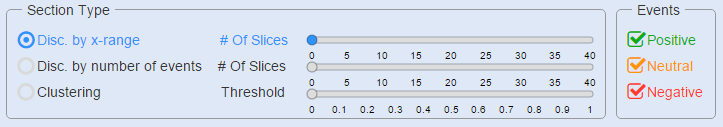
\includegraphics[width=130mm]{interaction_bar.png}
\caption{Interaction Bar for Summary Visualization}
\label{fig:interaction_bar}
\end{figure}
\section{General Interface}
Both the Session and Summary visualization are attached into an application which allows user to navigate different player and session. The interface of this application is divided into two areas: Navigation area and Visualization area\ref{fig:app_interface}. In Navigation area, user can choose patient and the sessions they have played. On clicking a session, a Session visualization of this session will be shown on the visualization area. It is also possible to open more than one Session visualization and rearrange the visualization window to compare gameplay between sessions. On clicking patient's name, Summary visualization for the chosen session will be shown.

\begin{figure}
\centering
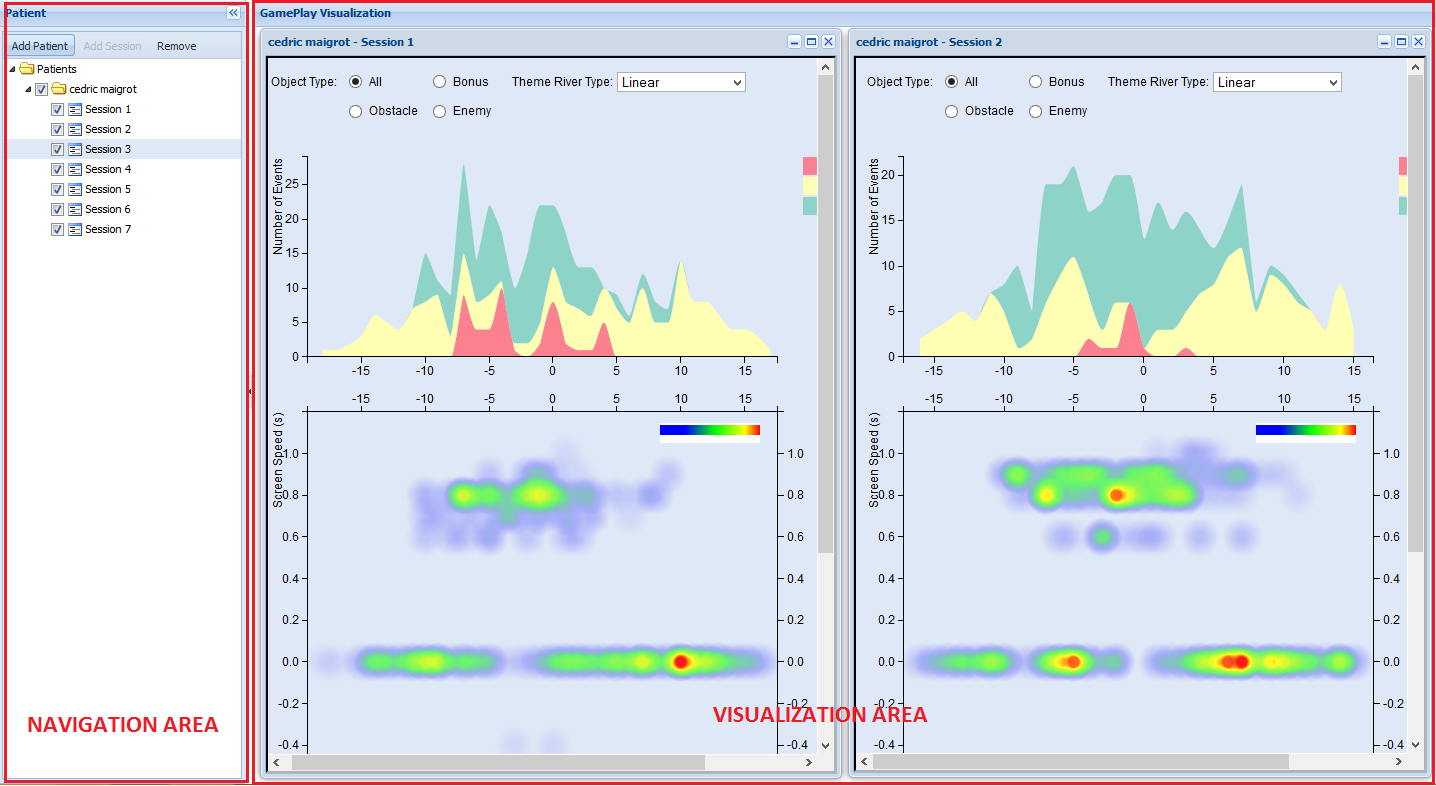
\includegraphics[width=150mm]{interface_app_compare.png}
\caption{Application Interface}
\label{fig:app_interface}
\end{figure}